
%%
%% Document class for CEUR-WS publications
%%
\documentclass[% 
% twocolumn,
% hf,
]{ceurart}

%%
%% The following packages are loaded automatically.
%%
\usepackage{amsmath}
\usepackage{amsfonts}
\usepackage{amssymb}
\usepackage{graphicx}
\usepackage{url}
\usepackage{listings}
\usepackage{subfig}
\usepackage{booktabs}
\usepackage{algorithm}
\usepackage[noend]{algpseudocode}

%% Additional packages for tables and units
\usepackage{multirow}
\usepackage{siunitx}

%%
%% It is recommended to use BibTeX to manage your references.
%%
\sloppy

%%
%% The document begins
%%
\begin{document}

%%
%% Copyright information
%%
\copyrightyear{2025}
\copyrightclause{Copyright for this paper by its authors.
  Use permitted under Creative Commons License Attribution 4.0
  International (CC BY 4.0).}

%%
%% Conference information
%%
\conference{IDDM'2025: 8th International Conference on Informatics \& Data-Driven Medicine, November 19--20, 2025, Lviv, Ukraine}

%%
%% The paper title
%%
\title{Architecture of Cyber-Physical Systems for UAV-Based Defect Detection in Photovoltaic Modules: Edge--Cloud YOLOv11 Thermography with RTK Geo-Indexing and SCADA-Aware Fire-Risk Logic}

%%
%% The author(s)
%%
\author[1]{Andrii Lysyi}
\author[2]{Anatoliy Sachenko}
\author[1]{Pavlo Radiuk}
\author[1]{Mykola Lysyi}
\author[1]{Oleksandr Melnychenko}
\author[1]{Oleg Savenko}
\cormark[1]

%%
%% The author's affiliation
%%
\address[1]{Khmelnytskyi National University, 11, Instytutska Str., Khmelnytskyi, 29016, Ukraine}
\address[2]{West Ukrainian National University, 11, Lvivska Str., Ternopil, 46009, Ukraine}

%%
%% The corresponding author text
%%
\cortext[1]{Corresponding author.}

%%
%% The abstract
%%
\begin{abstract}
Photovoltaic (PV) plants rely on infrared thermography to reveal cracks, delamination, soiling, and hotspot precursors, but many UAV inspection workflows remain offline, weakly geo-referenced, and poorly connected to plant supervision. In this work, we propose an edge--cloud cyber-physical architecture that couples smart UAV devices, an on-site edge server, and a cloud platform into a single operational loop. The UAV captures synchronized RGB and thermal frames and runs a lightweight YOLOv11 segmentation model on-board; the edge layer performs RTK-assisted geo-indexing and de-duplication, and issues SCADA-ready alarms through explicit fire-risk logic. On two benchmark thermogram representations (two- and three-color palettes) the on-board model achieves macro mAP@0.5 of 0.91 and 0.90, respectively, while late-fusion ensemble improves crack detection from 0.93 to 0.96 mAP@0.5 and reduces per-frame processing time from 4.235 s to 2.858 s. Field validation on rooftop and ground-mounted PV installations yields RMSE 0.71 between automatic and manual defect counts and shows strong sensitivity to flight settings, with 10 m altitude providing 93\% accuracy and 90\% recall. Overall, treating UAV inspection as a cyber-physical service---not a standalone detector---improves robustness, traceability, and operational usefulness for preventive maintenance and safety monitoring.
\end{abstract}

%%
%% Keywords
%%
\begin{keywords}
cyber-physical systems \sep
photovoltaic modules \sep
unmanned aerial vehicles \sep
infrared thermography \sep
edge computing \sep
deep learning segmentation \sep
SCADA integration
\end{keywords}

%%
%% Creates the title page
%%
\maketitle

\section{Introduction}
\label{sec:introduction}

Photovoltaic (PV) energy has moved from a niche technology to a critical component of modern power systems. At the same time, PV plants remain exposed to harsh outdoor environments and to a long list of failure modes that are mundane in origin but costly in aggregate. Microcracks can be introduced during manufacturing, transportation, installation, or hail events; they may evolve into inactive cell regions, hot spots, and power losses. Encapsulant aging and delamination can trap moisture and accelerate corrosion. Soiling reduces irradiance on the cells and changes the thermal regime, and damaged interconnects or bypass diodes can create abnormal heating that threatens safety. Reliability-centered maintenance is therefore not optional: predictive and preventive inspection directly affects energy yield and plant lifetime~\cite{TrikiLahiani2022RESS}.

Infrared (IR) thermography is one of the most informative non-contact diagnostic modalities for PV systems. It provides spatial maps of temperature that reflect electrical mismatch, increased series resistance, shunting, and local degradation. Reviews show that thermography can reveal a broad spectrum of PV anomalies but also highlight that its diagnostic value depends on acquisition conditions, emissivity assumptions, viewing geometry, and the ability to distinguish defect signatures from reflections and environmental gradients~\cite{Tsanakas2020Review,Rahman2020Review}. Comparative studies further demonstrate that defects may manifest differently under illumination and in dark conditions, which means that the inspection protocol is as important as the camera itself~\cite{GallardoSaavedra2020Sensors}.

Unmanned aerial vehicles (UAVs) have recently become the default platform for large-scale PV thermography. A UAV can cover utility-scale fields in minutes and can inspect rooftop installations that are difficult to access. Multiple studies report the operational benefits of UAV thermography, including improved coverage and reduced inspection time, but they also document practical constraints: flight altitude and speed control spatial resolution and motion blur; time of day and weather control thermal contrast; and specular reflections from the glass surface can produce misleading hot regions~\cite{Oliveira2020AerialIR,Hwang2021RemoteSensing,Marquez2022UAVCondition,LeePark2020Sensors}. These constraints are not merely nuisances; they are the reason why ``laboratory-grade'' image analysis pipelines often fail when deployed in the field.

Automation is the second major trend. Deep learning has achieved strong results in PV defect classification and localization across IR and RGB imagery, and surveys describe a rapidly growing set of architectures ranging from classical CNN classifiers to modern one-stage detectors and segmentation networks~\cite{Vergura2022Review,CardinaleVillalobos2023Sensors,Michail2024SciRep}. Recent UAV-oriented approaches use variants of the YOLO family to detect modules and anomalies in thermal and visible data~\cite{DiTommaso2022YOLOv3,Dey2024STYOLO}, and methods based on thermal video show that automation can be extended from single frames to temporal streams~\cite{Bommes2021IRVideo}. However, a recurring limitation is that many published methods implicitly assume an offline workflow: data are collected, uploaded, and processed in a batch manner. In operational PV plants, the inspection process is a closed-loop service that must satisfy latency, bandwidth, and reliability requirements, and it must deliver outputs that are traceable to physical modules and actionable by operators.

This observation motivates a systems-level framing. A PV inspection pipeline is not only a computer vision model; it is a cyber-physical system (CPS) in which sensing, computation, communication, and control are coupled. A UAV captures physical measurements, but the plant requires cyber actions: alarms, maintenance tickets, and safety procedures. Edge computing offers a natural architectural answer: it can reduce bandwidth by processing data near the source and can provide fast responses without depending on cloud connectivity~\cite{Shi2016EdgeComputing}. Yet, despite the maturity of edge computing in industrial monitoring, UAV inspection solutions for PV plants rarely provide an explicit CPS architecture that integrates on-board inference, edge aggregation, long-term cloud analytics, and SCADA-aware decision logic. Similarly, the literature on PV thermography tends to emphasize detection accuracy while under-reporting the geo-referencing and de-duplication steps required to avoid inflated counts and alarm fatigue.

The problem under consideration in this paper is therefore the design and validation of a CPS architecture for UAV-based PV defect monitoring that is accurate \emph{and} operationally actionable. The technical gap is not simply ``detect more defects'' but ``detect defects as part of a robust service'' with consistent geo-indexing, real-time execution on embedded hardware, and integration with plant supervision and safety monitoring. This is especially relevant for fire-risk mitigation, where abnormal heating and bypass diode failures can turn local defects into hazardous events. Integrating UAV-based detection with SCADA logic aligns with recent work that treats UAV and AI as components of plant safety monitoring pipelines~\cite{Lysyi2025EnhancedFire}.

The goal of this study is to improve the reliability, timeliness, and operational usefulness of UAV-based PV module inspection by developing a cyber-physical architecture that integrates on-board deep learning, edge computing, cloud analytics, and SCADA-aware decision logic into a single coordinated workflow.

To achieve this goal, the objective of this study is to design a method of operating a PV inspection CPS and to validate it experimentally under realistic flight and environmental conditions. The main scientific contributions are threefold:
\begin{itemize}
    \item We propose an explicit multi-tier CPS architecture (UAV--edge--cloud) for PV inspection that defines data flow, responsibilities, and decision points, including RTK-assisted geo-indexing and de-duplication to produce traceable, module-level defect events.
    \item We develop a thermography-oriented on-board inference pipeline based on YOLOv11 segmentation with palette-aware post-processing and late-fusion ensemble across two thermogram representations, achieving strong detection quality while reducing end-to-end processing time.
    \item We integrate detection outputs with an interpretable SCADA-aware logic layer for hazard inference, and we report field validation and sensitivity analysis with respect to flight parameters and environmental conditions to quantify operational robustness.
\end{itemize}

\section{Related Works}
\label{sec:related_works}

Research relevant to UAV-based PV defect monitoring spans sensing physics, computer vision, and systems engineering. This section briefly positions the present work within that landscape and clarifies how our focus on cyber-physical operation differs from detector-only contributions.

\paragraph{Thermography for PV diagnosis.}
Thermography is widely used to detect hot spots, mismatch, and degradation patterns in PV modules. Comprehensive reviews emphasize that thermal signatures are influenced by irradiance, ambient temperature, wind, and viewing angle, and they discuss recommended inspection procedures and limitations~\cite{Tsanakas2020Review,Rahman2020Review}. Gallardo-Saavedra \textit{et al.} compared illumination and dark conditions and showed that defect detectability depends on the operating state, which reinforces the need for consistent flight protocols and for contextual information such as irradiance and ambient conditions~\cite{GallardoSaavedra2020Sensors}. Practical UAV deployments have been evaluated in field studies that highlight how flight altitude and motion control affect spatial resolution and therefore anomaly separability~\cite{Oliveira2020AerialIR,LeePark2020Sensors}. These findings motivate our emphasis on flight-parameter sensitivity and reflection-aware planning.

\paragraph{Deep learning methods for PV defects.}
Deep learning for PV diagnostics has progressed from classification of cropped module images to detection and segmentation at the plant scale. Surveys summarize the expanding use of CNNs, object detectors, and hybrid models in PV monitoring~\cite{Vergura2022Review,CardinaleVillalobos2023Sensors}. Early work by Dotenco \textit{et al.} demonstrated automatic PV module detection and defect analysis in aerial infrared imagery using statistical tests and classical vision, reporting strong defect classification performance while also emphasizing the importance of robust pre-processing~\cite{Dotenco2016ECCV}. Later work increasingly relies on one-stage detectors. Di Tommaso \textit{et al.} proposed a multi-stage pipeline using YOLOv3 for module and anomaly detection in both IR and visible imagery, which improved automation but still required careful separation of tasks and datasets~\cite{DiTommaso2022YOLOv3}. Dey \textit{et al.} introduced ST-YOLO for PV fault detection from IR images and reported very high mAP@0.5 under their experimental conditions~\cite{Dey2024STYOLO}. Other studies focus on thermographic feature learning and robustness, including deep learning strategies for fault diagnosis from thermograms~\cite{Manno2021DLStrategies} and segmentation-based methods to delineate modules and defects~\cite{Henry2020Segmentation}. These works motivate our use of a segmentation-capable detector (YOLOv11-seg) and our attention to palette-induced domain shift.

\paragraph{Multi-modal inspection and contextual information.}
While thermography is central, many deployments use RGB imagery to provide context and reduce false alarms. RGB-based deep learning has been used to classify failure signatures and operational issues in PV plants~\cite{RicoEspinosa2020FailureSignature}. Multi-modal pipelines can also support human interpretability, because operators can inspect RGB context when thermal signatures are ambiguous. Our architecture therefore assumes synchronized RGB and thermal acquisition, even though the defect detector in this paper focuses on thermal masks.

\paragraph{Edge--cloud architectures and cyber-physical integration.}
From a systems perspective, UAV inspection is an instance of distributed sensing with stringent constraints. Edge computing is often advocated for industrial IoT because it reduces cloud dependence and provides low-latency decisions~\cite{Shi2016EdgeComputing}. Tang \textit{et al.} demonstrated an edge--cloud deep learning architecture for detecting linear defects in large-scale PV plants, showing that distributed computation can support plant-scale monitoring and reduce data transfer~\cite{Tang2022EdgeCloud}. However, many edge--cloud works stop at ``detection at the edge'' and do not explicitly model the feedback loop to plant operations. Our work extends this direction by adding RTK-based geo-indexing, duplicate suppression, and SCADA-aware fire-risk logic, motivated by the observation that PV defects have both performance and safety implications~\cite{Lysyi2025EnhancedFire}.

\paragraph{Objective and tasks.}
The objective of this study is to develop and validate an end-to-end CPS architecture for UAV-based PV defect monitoring that is accurate, geo-referenced, and actionable. To fulfill this objective, three tasks must be completed: (1) formalize the UAV--edge--cloud architecture and define interfaces for data, geo-tags, and alarms; (2) develop and validate an on-board thermography detection pipeline with palette-aware post-processing and fusion; and (3) perform quantitative evaluation and field validation, including sensitivity analysis to operational conditions, to assess whether the architecture improves real inspection workflows rather than only offline metrics.

\section{Methods}
\label{sec:methods}

This section details the proposed approach titled ``Architecture of Cyber-Physical Systems for UAV-Based Defect Detection in Photovoltaic Modules.'' We describe the CPS architecture, sensing and communication design, reflection-aware flight planning, dataset construction, on-board deep learning inference, edge/cloud analytics, and the SCADA-aware decision layer. The guiding principle is to treat defect detection as a cyber-physical workflow: sensing, computation, communication, and action must be co-designed.

\subsection{System Architecture and Operational Loop}
\label{subsec:architecture}

\begin{figure}[!ht]
    \centering
    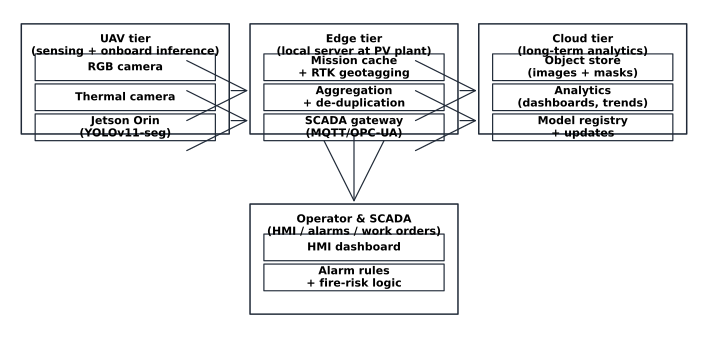
\includegraphics[width=1.0\linewidth]{figs/cps_architecture.pdf}
    \caption{Proposed cyber-physical architecture for UAV-based PV defect monitoring. The UAV tier performs synchronized sensing and on-board YOLOv11 segmentation. The edge tier aggregates detections, performs RTK-based geo-indexing and de-duplication, and interfaces with SCADA. The cloud tier provides long-term storage, analytics, and model lifecycle management.}
    \label{fig:cps_architecture}
\end{figure}

We operationalize PV inspection as a closed loop that starts with sensing and ends with a plant-level action. The CPS is organized into three computational tiers (Figure~\ref{fig:cps_architecture}): the UAV tier, the edge tier deployed at the PV plant, and the cloud tier for long-term analytics. An operator layer interacts with the CPS through a dashboard and through SCADA/HMI interfaces.

The UAV tier is responsible for time-critical tasks. It captures synchronized RGB and thermal frames and performs on-board inference to produce defect candidates. The edge tier is responsible for plant-context tasks: it performs RTK-assisted geo-indexing, de-duplicates repeated detections, aggregates them into module-level events, and interfaces with SCADA for alarms and maintenance triggers. The cloud tier stores mission data, supports retrospective analytics and reporting, and hosts model lifecycle services (e.g., model registry and updates). This tiering reflects practical constraints: streaming raw thermal video to the cloud is bandwidth-intensive, while running full analytics on-board is constrained by embedded compute and power.

Let a mission produce a time-ordered stream of frames $\{I_t\}_{t=1}^{T}$, where each frame contains an RGB image $I_t^{\mathrm{rgb}}$, a thermal image $I_t^{\mathrm{th}}$, and a navigation record $n_t$ (RTK position, altitude, yaw, and timestamp). On-board inference produces a set of detections:
\begin{equation}
\mathcal{D}_t = \{(c_k, M_k, s_k, g_k)\}_{k=1}^{K_t},
\label{eq:detections}
\end{equation}
where $c_k$ is the defect class (crack, soiling, delamination), $M_k$ is a segmentation mask, $s_k$ is a confidence score, and $g_k$ is a geo-tag (estimated module location in plant coordinates). The edge server receives $\mathcal{D}_t$ and performs (i) spatial clustering and de-duplication across time, (ii) association of detections with module identifiers and strings, and (iii) state inference that maps detections and SCADA signals to operational actions. The cloud stores mission artifacts and provides dashboards for trend analysis, module history, and inspection reporting.

\subsection{UAV Platform, Sensors, and Communication}
\label{subsec:platform}

The CPS assumes a UAV platform capable of stable flight in predefined patterns (grid or corridor scanning) and equipped with a combined RGB/thermal payload. The thermal channel provides the primary signal for anomalous heating patterns; the RGB channel provides contextual information and supports operator validation. While the architecture is platform-agnostic, the reported implementation is comparable to Matrice-class UAVs with a dual-sensor gimbal payload (RGB + thermal) and RTK positioning. 

From a CPS viewpoint, geo-referencing is as important as imaging. RTK positioning reduces drift and enables consistent mapping of detections to physical modules across missions. In addition, accurate timestamps allow synchronization between the thermal camera, the RGB camera, and the flight controller. We assume that the UAV logs the navigation record $n_t$ for each frame, including RTK position and altitude. This record is later used for de-duplication and for associating detections with the plant layout.

Communication is treated as a constrained resource. Streaming full-resolution thermal video is often infeasible over standard UAV links, especially in large plants. Instead, the UAV transmits compact detection messages (Eq.~\eqref{eq:detections}) to the edge server in near-real time. Full-resolution images may be cached on-board and uploaded post-flight or selectively uploaded when the edge server requests evidence. This design follows the general rationale for edge computing in industrial monitoring: local inference reduces bandwidth, and plant-level decisions can be made without dependence on cloud connectivity~\cite{Shi2016EdgeComputing}.

\subsection{Reflection-Aware Viewpoint Selection}
\label{subsec:flightplanning}

UAV thermography of PV modules is vulnerable to specular reflections from the glass surface. If the camera view aligns with the specular reflection direction of the sun, the thermogram can be dominated by glare, producing false hotspots and corrupting the thermal contrast needed for defect detection. To mitigate this, we incorporate a reflection-aware viewpoint selection method that uses RTK geometry and the solar position.

\begin{figure}[!ht]
    \centering
    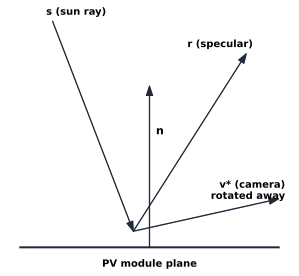
\includegraphics[width=.85\linewidth]{figs/glare_geometry.pdf}
    \caption{Geometric intuition for reflection-aware viewpoint selection. Given the module plane normal $n$ and the solar ray direction $s$, the specular reflection direction $r$ is computed. The desired camera viewing direction $v^\star$ is obtained by rotating away from $r$ (Rodrigues rotation) to reduce glare while maintaining sufficient incidence for thermal contrast.}
    \label{fig:glare_geometry}
\end{figure}

Let three RTK-referenced points on the module plane be $p_1, p_2, p_3 \in \mathbb{R}^3$ (e.g., corners of a representative module). The module normal vector is computed as
\begin{equation}
n = \frac{(p_2-p_1)\times(p_3-p_1)}{\|(p_2-p_1)\times(p_3-p_1)\|}.
\label{eq:normal}
\end{equation}
Let $s$ be the unit vector pointing from the module to the sun (obtained from a solar ephemeris model at timestamp $t$). The specular reflection direction is
\begin{equation}
r = s - 2(n^\top s)\,n.
\label{eq:reflection}
\end{equation}
If the camera viewing direction aligns with $r$, specular reflections dominate. We therefore define a target viewing direction $v^\star$ by rotating $r$ around the normal $n$ by an angle $\theta$ selected so that the reflection direction falls outside the camera field of view. Using Rodrigues' rotation formula, the rotated vector is
\begin{equation}
v^\star = r\cos\theta + (n\times r)\sin\theta + n(n^\top r)(1-\cos\theta).
\label{eq:rodrigues}
\end{equation}

Algorithm~\ref{alg:glare} summarizes this viewpoint selection procedure. In practice, $\Theta$ can be a small set of candidate angles (e.g., $\pm 5^\circ, \pm 10^\circ$) and the glare score can be approximated by the angular distance between $v_\theta$ and $r$ relative to the camera field of view. The key point is that the method is lightweight and compatible with real-time decision-making at the edge tier.

\begin{algorithm}[!ht]
\caption{Reflection-aware viewpoint selection for UAV thermography}
\label{alg:glare}
\begin{algorithmic}[1]
\Require RTK plane points $p_1,p_2,p_3$, solar direction $s$, candidate rotation angles $\Theta$
\Ensure View direction $v^\star$ that reduces specular glare
\State Compute surface normal $n$ using Eq.~\eqref{eq:normal}
\State Compute reflection direction $r$ using Eq.~\eqref{eq:reflection}
\ForAll{$\theta \in \Theta$}
    \State Compute candidate view $v_\theta$ using Eq.~\eqref{eq:rodrigues}
    \State Evaluate a glare score (expected reflection within camera FOV)
\EndFor
\State Select $v^\star = \arg\min_{\theta} \mathrm{GlareScore}(v_\theta)$
\State \Return $v^\star$
\end{algorithmic}
\end{algorithm}

\subsection{Thermogram Representations and Dataset Construction}
\label{subsec:dataset}

Thermal cameras often support multiple color palettes that map temperature ranges to colors for visualization. While these palettes are designed for human interpretation, they also change the statistical distribution of pixel values presented to a learning model. In our experiments we consider two thermogram representations: a two-color palette (denoted \textbf{M2}) and a three-color palette (denoted \textbf{M3}). The key difference is the effective temperature range emphasized by the rendering. In the reported setup, M3 uses a narrower dynamic range of approximately 15\,$^{\circ}$C, which increases sensitivity to small temperature contrasts (on the order of 0.1--0.5\,$^{\circ}$C) but can saturate extreme anomalies. M2 uses a wider range of approximately 35\,$^{\circ}$C, which reduces sensitivity to tiny hot spots but covers the full spectrum from mild mismatch heating to severe damage. We treat M2 and M3 as two benchmark thermogram representations derived from the same physical scenes to evaluate robustness to palette-induced domain differences and to motivate selective fusion.

A supervised dataset was constructed from field thermography and complementary public images. Images were annotated for three defect classes relevant to preventive maintenance: \textit{crack}, \textit{soiling}, and \textit{delamination}. Annotations were produced using the Computer Vision Annotation Tool (CVAT)~\cite{Sekachev2020CVAT} and exported as polygon masks suitable for segmentation training. The dataset size is modest (200 images), but it reflects realistic constraints for domain-specific inspection problems: collecting high-quality thermal data under suitable irradiance and ensuring correct labeling requires expertise and careful field work.

Table~\ref{tab:dataset_structure} reports the dataset composition and the train/validation/test split. The class distribution is imbalanced, with delamination dominating. This is typical in field monitoring where some defect types are frequent while others are rare but high-impact. The imbalance motivates the use of segmentation masks and careful post-processing, because minority classes can otherwise be overwhelmed by false positives.

\begin{table}[!ht]
\centering
\caption{Dataset structure and split used for training and evaluation.}
\label{tab:dataset_structure}
\small
\begin{tabular}{lcccc}
\toprule
\textbf{Class} & \textbf{Defect type} & \textbf{Total images} & \textbf{Train/Val/Test (\%)} & \textbf{Train/Val/Test (count)}\\
\midrule
1 & Crack & 20 & 80/10/10 & 16/2/2 \\
2 & Soiling & 10 & 80/10/10 & 8/1/1 \\
3 & Delamination & 170 & 80/10/10 & 136/17/17 \\
\midrule
\multicolumn{2}{l}{\textbf{Total}} & \textbf{200} &  & 160/20/20 \\
\bottomrule
\end{tabular}
\end{table}

\subsection{On-Board Deep Learning: YOLOv11 Segmentation}
\label{subsec:yolo}

The UAV tier runs a lightweight deep learning model for defect detection and segmentation. We choose a YOLO-family segmentation model because it offers a strong accuracy--speed trade-off and has mature deployment tooling. Specifically, YOLOv11-seg is used as the core network~\cite{Ultralytics2025}. The model outputs bounding boxes and pixel-level masks for each detected defect. Masks are valuable in PV inspection because they enable estimation of defect area and shape, which improves prioritization and supports temporal tracking.

The detector is trained on the annotated dataset described in Table~\ref{tab:dataset_structure}. During inference, the model produces a set of candidate instances $\{(b_k, M_k, s_k, c_k)\}$, where $b_k$ is a bounding box and $M_k$ is a mask. Non-maximum suppression (NMS) removes duplicate boxes, and an analogous mask-level suppression is applied to reduce overlapping instance masks. The post-processing stage is particularly important because UAV video streams contain multiple near-duplicate frames, and thermal palettes can produce color artifacts that trigger spurious detections.

\subsection{Mask Similarity, Size-Based Routing, and Post-Processing}
\label{subsec:postprocessing}

On-board inference yields instance masks, which must be filtered and merged to produce stable defect events. We use mask overlap based on intersection-over-union (IoU):
\begin{equation}
\mathrm{IoU}(A,B) = \frac{|A\cap B|}{|A\cup B|}.
\label{eq:iou}
\end{equation}
Mask-level suppression (Mask-NMS) removes duplicate instances when IoU exceeds a threshold, retaining the higher-confidence prediction. Mask-NMS is important in UAV inspection because adjacent frames often contain the same defect with slightly shifted masks.

Beyond duplicate suppression, the CPS performs \emph{size-based routing} of defect instances between the two thermogram representations. Let $S_{\mathrm{def}}$ denote the area (in pixels) of a detected defect mask, and let $S_{\mathrm{cell}}$ denote the area of a single PV cell in the same image scale. We define the relative defect area
\begin{equation}
R_d = \frac{S_{\mathrm{def}}}{S_{\mathrm{cell}}}.
\label{eq:rd_ratio}
\end{equation}
The intuition is that defects smaller than one cell behave like localized hot spots and benefit from the higher contrast of M3, whereas larger anomalies are more reliably represented in the wider-range M2 thermogram.

Using $R_d$, we form two mutually exclusive defect sets:
\begin{equation}
\mathcal{D}_{\mathrm{small}} = \{ d \in \mathcal{D}^{\mathrm{M3}} \mid R_d(d) < 1.0 \},
\label{eq:dsmall}
\end{equation}
\begin{equation}
\mathcal{D}_{\mathrm{large}} = \{ d \in \mathcal{D}^{\mathrm{M2}} \mid R_d(d) \ge 1.0 \},
\label{eq:dlarge}
\end{equation}
and the final set of detections is
\begin{equation}
\mathcal{D}_{\mathrm{final}} = \mathcal{D}_{\mathrm{small}} \cup \mathcal{D}_{\mathrm{large}}.
\label{eq:dfinal}
\end{equation}
Because the routing criteria are complementary and Mask-NMS is applied within each branch, the resulting sets satisfy $\mathcal{D}^{\mathrm{M3}}\cap \mathcal{D}^{\mathrm{M2}}=\varnothing$ in practice, and duplicate alarms are reduced. In the technical report, applying Mask-NMS and selective combination reduced false triggers by approximately 8\% in field-like sequences.

We distinguish two palette-specific post-processing pipelines.

\paragraph{M3 processing (three-color palette).}
The three-color palette increases sensitivity to small anomalies but can introduce banding. The M3 branch therefore targets small defects (Eq.~\eqref{eq:dsmall}) and uses a conservative IoU threshold (0.4) in Mask-NMS. Algorithm~\ref{alg:m3} summarizes the steps.

\begin{algorithm}[!ht]
\caption{On-board processing of a three-color thermogram (M3)}
\label{alg:m3}
\begin{algorithmic}[1]
\Require Thermogram $I^{\mathrm{th}}$ in three-color palette, YOLOv11-seg model, thresholds $(\tau_c,\tau_{\mathrm{IoU}})$
\Ensure Filtered defect set $\mathcal{D}_{\mathrm{small}}$
\State Convert thermogram to a multi-channel representation (palette split)
\State Run YOLOv11-seg to obtain candidate masks and confidences
\State Apply confidence filtering: keep masks with $s_k \ge \tau_c$ (e.g., $\tau_c=0.25$)
\State Compute $R_d$ for each mask using Eq.~\eqref{eq:rd_ratio}; keep only instances with $R_d<1.0$
\State Apply Mask-NMS using IoU threshold $\tau_{\mathrm{IoU}}$ (e.g., 0.4)
\State Geo-tag detections using RTK navigation record $n_t$
\State \Return $\mathcal{D}_{\mathrm{small}}$
\end{algorithmic}
\end{algorithm}

\paragraph{M2 processing (two-color palette).}
The two-color palette covers a wider temperature range and supports detection of larger anomalies. The M2 branch targets large defects (Eq.~\eqref{eq:dlarge}) and uses a slightly higher Mask-NMS IoU threshold (0.5). Algorithm~\ref{alg:m2} gives the steps.

\begin{algorithm}[!ht]
\caption{On-board processing of a two-color thermogram (M2)}
\label{alg:m2}
\begin{algorithmic}[1]
\Require Thermogram $I^{\mathrm{th}}$ in two-color palette, YOLOv11-seg model
\Ensure Filtered defect set $\mathcal{D}_{\mathrm{large}}$
\State Normalize thermogram and run YOLOv11-seg
\State Apply confidence filtering and Mask-NMS (IoU threshold 0.5)
\State Compute $R_d$ for each mask using Eq.~\eqref{eq:rd_ratio}; keep only instances with $R_d\ge 1.0$
\State Geo-tag detections using RTK navigation record $n_t$
\State \Return $\mathcal{D}_{\mathrm{large}}$
\end{algorithmic}
\end{algorithm}

\subsection{Late-Fusion Ensemble Across Thermogram Representations}

\label{subsec:ensemble}

Palette-induced domain differences motivate model fusion. Rather than training a large multi-domain model, we implement a lightweight late-fusion ensemble based on the size-routed branches defined in Eqs.~\eqref{eq:dsmall}--\eqref{eq:dfinal}. The detector is applied to both representations, producing $\mathcal{D}_t^{\mathrm{M2}}$ and $\mathcal{D}_t^{\mathrm{M3}}$, and the edge tier combines them by the set-union rule:
\begin{equation}
\mathcal{D}_t^{\mathrm{ens}} \equiv \mathcal{D}_{\mathrm{final}} = \mathcal{D}_{\mathrm{small}} \cup \mathcal{D}_{\mathrm{large}},
\label{eq:ensemble}
\end{equation}
This selective fusion keeps the branch that is best suited to the expected thermal contrast regime: M3 contributes the small-defect set, and M2 contributes the large-defect set. The edge tier further suppresses duplicates across frames using RTK geo-indexing (Section~\ref{subsec:dedup}). The design is compatible with real-time operation because it does not require joint training or a heavier backbone; the additional cost is limited to running the detector on two representations.

\subsection{Edge-Level Geo-Indexing and De-Duplication}
\label{subsec:dedup}

A UAV mission produces repeated observations of the same modules across consecutive frames and overlapping flight lines. Without de-duplication, a single defect can be counted many times, inflating alarms and reducing operator trust. We therefore perform RTK-assisted geo-indexing and de-duplication at the edge tier.

Each detection in $\mathcal{D}_t$ is mapped to an approximate module location using the UAV RTK position, altitude, and camera geometry. The exact projection depends on camera calibration and gimbal orientation; in our implementation we use a simplified mapping sufficient for clustering at module granularity, and we refine association using the plant layout map.

To compute distances between geo-tagged detections, we use the Haversine distance between latitude/longitude coordinates:
\begin{equation}
d = 2R \arcsin\!\left(\sqrt{\sin^2\!\left(\frac{\Delta\varphi}{2}\right)+\cos\varphi_1\cos\varphi_2\sin^2\!\left(\frac{\Delta\lambda}{2}\right)}\right),
\label{eq:haversine}
\end{equation}
where $R$ is the Earth radius, $\varphi$ is latitude, and $\lambda$ is longitude. Detections are clustered using a distance threshold $\epsilon$ derived from the ground sampling distance and expected RTK error. Within each cluster, the edge server aggregates detections over time, retains representative evidence frames, and associates the cluster to a module ID or string based on the plant layout. The result is a set of module-level defect events rather than frame-level detections.

\subsection{SCADA-Aware State Inference and Fire-Risk Logic}
\label{subsec:scada}

Defect detection becomes operationally useful when it maps to plant-level actions. Our CPS includes a decision layer that combines UAV detections with electrical and supervisory signals to infer operating states and hazard conditions. The core idea is to express safety-relevant conditions in interpretable logic that can be audited by engineers and integrated into SCADA rule engines.

We define binary variables $X_1, X_2, X_3$ that indicate the presence of a defect in strings 1--3 of a module group (or a comparable partition of the electrical layout). Variables $X_{11}, X_{12}, X_{13}$ indicate whether bypass diodes in the corresponding strings operate correctly (1 indicates correct operation). The hazard output $Y$ is defined as
\begin{equation}
Y = X_1 \overline{X_{11}} + X_2 \overline{X_{12}} + X_3 \overline{X_{13}},
\label{eq:fire_logic}
\end{equation}
which captures the engineering intuition that defects combined with failed bypass diodes increase overheating risk. The full truth table used in the technical report is summarized in Table~\ref{tab:truth_table}.

To incorporate additional safety sensors (e.g., smoke or flame detectors), we add binary variables $X_{21}, X_{22}$ representing sensor triggers. The extended hazard logic is
\begin{equation}
Y = X_1 \overline{X_{11}} + X_2 \overline{X_{12}} + X_3 \overline{X_{13}} + X_1 X_{21} + X_2 X_{22}.
\label{eq:fire_logic_ext}
\end{equation}
The edge server evaluates these expressions in real time and forwards alarms to the SCADA/HMI layer, where standard procedures (e.g., dispatch, shutdown recommendation) can be executed.

\begin{table}[!ht]
\centering
\caption{Truth table for module operating state and hazard output $Y$ (excerpted and translated). $X_1$--$X_3$ indicate defects in three strings; $X_{11}$--$X_{13}$ indicate bypass diode correctness; $Y=1$ denotes a hazardous state.}
\label{tab:truth_table}
\scriptsize
\setlength{\tabcolsep}{3pt}
\begin{tabular}{ccccccccl}
\toprule
\textbf{\#} & $X_1$ & $X_2$ & $X_3$ & $X_{11}$ & $X_{12}$ & $X_{13}$ & $Y$ & \textbf{State description} \\
\midrule
1  & 0 & 0 & 0 & 0 & 0 & 0 & 0 & normal operation \\
2  & 0 & 0 & 0 & 0 & 0 & 1 & 0 & normal operation \\
3  & 0 & 0 & 0 & 0 & 1 & 0 & 0 & normal operation \\
4  & 0 & 0 & 0 & 0 & 1 & 1 & 0 & normal operation \\
5  & 0 & 0 & 0 & 1 & 0 & 0 & 0 & normal operation \\
6  & 0 & 0 & 0 & 1 & 0 & 1 & 0 & normal operation \\
7  & 0 & 0 & 0 & 1 & 1 & 0 & 0 & normal operation \\
8  & 0 & 0 & 0 & 1 & 1 & 1 & 0 & normal operation \\
9  & 1 & 0 & 0 & 0 & 0 & 0 & 1 & hazard; bypass diode failure \\
10 & 0 & 1 & 0 & 0 & 0 & 0 & 1 & hazard; bypass diode failure \\
11 & 0 & 0 & 1 & 0 & 0 & 0 & 1 & hazard; bypass diode failure \\
12 & 1 & 1 & 0 & 0 & 0 & 0 & 1 & hazard; bypass diode failure \\
13 & 1 & 0 & 1 & 0 & 0 & 0 & 1 & hazard; bypass diode failure \\
14 & 0 & 1 & 1 & 0 & 0 & 0 & 1 & hazard; bypass diode failure \\
15 & 1 & 1 & 1 & 0 & 0 & 0 & 1 & hazard; bypass diode failure \\
16 & 1 & 0 & 0 & 1 & 0 & 0 & 0 & bypass diode blocks string \\
17 & 0 & 1 & 0 & 0 & 1 & 0 & 0 & bypass diode blocks string \\
18 & 0 & 0 & 1 & 0 & 0 & 1 & 0 & bypass diode blocks string \\
19 & 1 & 1 & 1 & 1 & 1 & 1 & 0 & bypass diodes block strings \\
20 & 1 & 0 & 1 & 1 & 0 & 1 & 0 & bypass diodes block strings \\
\bottomrule
\end{tabular}
\end{table}

\subsection{Temperature Context via NOCT Approximation}
\label{subsec:noct}

To interpret thermal anomalies, the CPS can optionally estimate expected module temperature under nominal conditions using the Nominal Operating Cell Temperature (NOCT) approximation. Given ambient temperature $T_{\mathrm{amb}}$ and irradiance $G$ (W/m$^2$), the expected module temperature is approximated by
\begin{equation}
T_m = T_{\mathrm{amb}} + \frac{\mathrm{NOCT}-20}{800}\,G.
\label{eq:noct}
\end{equation}
This estimate is not a replacement for thermography; it provides context for whether observed temperatures are plausible under current irradiance and weather conditions, which can help to flag cases where reflections or transient shading dominate.

\subsection{Experimental Metrics}
\label{subsec:metrics}

Defect detection performance is evaluated using standard metrics. For a given class, precision and recall are defined as
\begin{equation}
\mathrm{Precision} = \frac{TP}{TP+FP}, \qquad
\mathrm{Recall} = \frac{TP}{TP+FN},
\label{eq:pr}
\end{equation}
where $TP$, $FP$, and $FN$ denote true positives, false positives, and false negatives. Detection quality is summarized by average precision (AP) and mean average precision (mAP). We report mAP@0.5, i.e., AP computed at IoU threshold 0.5 and averaged across classes. For field validation against manual monitoring, we report the root mean squared error (RMSE) between automatic and manual defect counts:
\begin{equation}
\mathrm{RMSE} = \sqrt{\frac{1}{N}\sum_{i=1}^{N}(y_i-\hat{y}_i)^2}.
\label{eq:rmse}
\end{equation}

Operational performance is characterized by inference throughput (frames per second), end-to-end processing time, and sensitivity to flight and environmental parameters (altitude, speed, time of day, weather). Sensitivity analysis is essential because a method that only works in a narrow operating envelope is unlikely to be adopted in real PV plants.

\section{Results}
\label{sec:results}

This section reports quantitative results for the proposed CPS-enabled defect detection pipeline. We focus on real data experiments and exclude synthetic experiments. Results are organized into (i) detection quality on two thermogram representations (M2 and M3), (ii) the effect of ensemble fusion, (iii) edge hardware considerations and YOLO model comparison, (iv) field validation against manual inspection, and (v) sensitivity to flight and weather parameters.

\subsection{Detection Quality on Two Benchmark Thermogram Representations}
\label{subsec:results_m2m3}

Tables~\ref{tab:m2_perf} and~\ref{tab:m3_perf} summarize per-class results for YOLOv11-seg on M2 and M3. On the two-color palette (M2), the model achieves macro mAP@0.5 of 0.91, precision of 0.89, and recall of 0.87. On the three-color palette (M3), macro mAP@0.5 is 0.90 with precision 0.88 and recall 0.86. These averages are close, but class-wise behavior differs. Crack detection is stronger on M2 (mAP@0.5 0.93) than on M3 (0.87), while delamination detection is strongest on M3 (0.93). This pattern supports the practical claim that thermogram palettes act as distinct domains and that a single representation may emphasize some defect signatures at the expense of others.

\begin{table}[!ht]
\centering
\caption{Performance on thermogram M2 (two-color palette) using YOLOv11-seg.}
\label{tab:m2_perf}
\small
\begin{tabular}{lccc}
\toprule
\textbf{Class} & \textbf{mAP@0.5} & \textbf{Precision} & \textbf{Recall} \\
\midrule
Crack & 0.93 & 0.91 & 0.89 \\
Soiling & 0.90 & 0.88 & 0.86 \\
Delamination & 0.89 & 0.87 & 0.85 \\
\midrule
\textbf{Macro average} & \textbf{0.91} & \textbf{0.89} & \textbf{0.87} \\
\bottomrule
\end{tabular}
\end{table}

\begin{table}[!ht]
\centering
\caption{Performance on thermogram M3 (three-color palette) using YOLOv11-seg.}
\label{tab:m3_perf}
\small
\begin{tabular}{lccc}
\toprule
\textbf{Class} & \textbf{mAP@0.5} & \textbf{Precision} & \textbf{Recall} \\
\midrule
Crack & 0.87 & 0.86 & 0.84 \\
Soiling & 0.90 & 0.88 & 0.86 \\
Delamination & 0.93 & 0.90 & 0.88 \\
\midrule
\textbf{Macro average} & \textbf{0.90} & \textbf{0.88} & \textbf{0.86} \\
\bottomrule
\end{tabular}
\end{table}

\begin{figure}[!ht]
  \centering
  \subfloat[Two-color palette (M2)]{\includegraphics[width=.48\linewidth]{figs/map_m2.pdf}\label{fig:map_m2}}
  \hfill
  \subfloat[Three-color palette (M3)]{\includegraphics[width=.48\linewidth]{figs/map_m3.pdf}\label{fig:map_m3}}
  \caption{Detection quality (mAP@0.5) for YOLOv11-seg on two thermogram representations. The palette choice changes class-wise behavior, motivating late-fusion ensemble.}
  \label{fig:map_models}
\end{figure}

\subsection{Effect of Late-Fusion Ensemble and Runtime Impact}
\label{subsec:results_ensemble}

Late-fusion ensemble improves robustness without requiring a heavier network. Table~\ref{tab:ensemble} reports mAP@0.5 before and after fusion. The crack class benefits most, improving from 0.93 to 0.96 mAP@0.5. This matters operationally because crack-like patterns can be subtle and can be confounded by thermal noise or reflections. Delamination improves from 0.93 to 0.95, while soiling remains stable. Figure~\ref{fig:ensemble_gain} visualizes these changes.

The ensemble pipeline also improves runtime. By merging detections early and avoiding repeated post-processing, the reported per-frame processing time was reduced from 4.235\,s to 2.858\,s. Although this latency depends on hardware and implementation, the reduction illustrates that careful pipeline design can improve both accuracy and operational responsiveness, which is critical for CPS operation.

\begin{table}[!ht]
\centering
\caption{Ensemble fusion effect on mAP@0.5 (before vs. after).}
\label{tab:ensemble}
\small
\begin{tabular}{lcc}
\toprule
\textbf{Class} & \textbf{Before} & \textbf{After ensemble} \\
\midrule
Crack & 0.93 & 0.96 \\
Soiling & 0.90 & 0.90 \\
Delamination & 0.93 & 0.95 \\
\bottomrule
\end{tabular}
\end{table}

\begin{figure}[!ht]
\centering
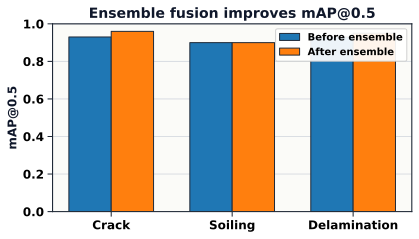
\includegraphics[width=.75\linewidth]{figs/ensemble_gain.pdf}
\caption{mAP@0.5 improvements after late-fusion ensemble of M2 and M3 detections.}
\label{fig:ensemble_gain}
\end{figure}

\subsection{Edge Hardware and YOLO Model Comparison}
\label{subsec:results_hw}

Deploying deep learning on UAVs imposes strict constraints on compute, weight, and power. Table~\ref{tab:hardware} summarizes representative embedded platforms and highlights a practical trade-off: throughput controls the maximum feasible flight speed and frame rate, while detection quality can depend on available accelerators and supported precision.

The NVIDIA Jetson Orin Nano achieves the highest throughput (100 FPS) and the best reported mAP@0.5 (0.95), making it suitable for on-board inference with segmentation. Lower-power systems such as Ambarella H2 and Qualcomm QCS605 offer alternatives but with reduced mAP@0.5. Figure~\ref{fig:hardware_tradeoff} visualizes the throughput--quality relationship.

\begin{table}[!ht]
\centering
\caption{Representative edge hardware comparison for on-board inference.}
\label{tab:hardware}
\small
\begin{tabular}{lccc}
\toprule
\textbf{Platform} & \textbf{Throughput (FPS)} & \textbf{mAP@0.5} & \textbf{Precision} \\
\midrule
NVIDIA Jetson Orin Nano & 100 & 0.95 & 0.93 \\
Ambarella H2 & 60 & 0.70 & 0.75 \\
Qualcomm QCS605 & 80 & 0.85 & 0.82 \\
\bottomrule
\end{tabular}
\end{table}

\begin{figure}[!ht]
\centering
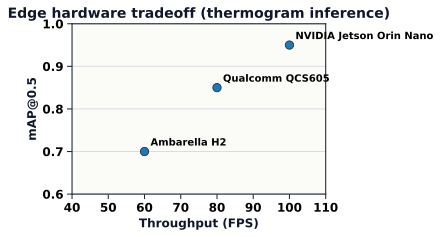
\includegraphics[width=.75\linewidth]{figs/hardware_tradeoff.pdf}
\caption{Throughput vs. detection quality trade-off for representative embedded platforms.}
\label{fig:hardware_tradeoff}
\end{figure}

To further justify the choice of YOLOv11, we trained and evaluated several YOLO generations under a consistent protocol. Table~\ref{tab:yolo_compare} reports precision, recall, and mAP@0.5, along with training time. YOLOv11 achieves the strongest overall performance (precision 0.96, recall 0.95, mAP@0.5 0.93), albeit with longer training time than some smaller models. The result suggests that, for on-board inference, YOLOv11 provides a favorable balance between accuracy and manageable deployment complexity.

\begin{table}[!ht]
\centering
\caption{Quantitative comparison of YOLO model generations (segmentation).}
\label{tab:yolo_compare}
\small
\begin{tabular}{lcccc}
\toprule
\textbf{Model} & \textbf{Precision} & \textbf{Recall} & \textbf{mAP@0.5} & \textbf{Training time (min)} \\
\midrule
YOLOv5 & 0.92 & 0.90 & 0.86 & 55 \\
YOLOv8 & 0.91 & 0.88 & 0.83 & 45 \\
YOLOv9 & 0.94 & 0.80 & 0.90 & 59 \\
YOLOv10 & 0.94 & 0.86 & 0.90 & 132 \\
YOLOv11 & \textbf{0.96} & \textbf{0.95} & \textbf{0.93} & 106 \\
\bottomrule
\end{tabular}
\end{table}

\subsection{Field Validation Against Manual Monitoring}
\label{subsec:results_field}

A CPS intended for plant operation must agree with human inspection under field conditions. We validated the CPS output against manual monitoring on two PV installations: a rooftop plant and a ground-mounted plant. The evaluation compares automatic defect counts after edge-level de-duplication with manual counts obtained by expert review. The technical report reports RMSE of 0.71 (Eq.~\eqref{eq:rmse}) across monitored module groups, indicating that the CPS produces defect counts close to human assessment.

Beyond aggregate error, field testing highlights the role of CPS components that are not visible in offline metrics. On-board inference alone produces repeated detections for the same defect across adjacent frames; RTK-based clustering and de-duplication at the edge tier reduce this redundancy and produce module-level events suitable for reporting. Similarly, when abnormal heating is detected, the SCADA-aware logic can elevate the event priority, especially if bypass diode status indicates increased risk. These elements are essential for operational adoption because operators need stable counts, clear module identifiers, and actionable alerts rather than a stream of raw detections.

\subsection{Sensitivity to Flight and Environmental Parameters}
\label{subsec:results_sensitivity}

Thermographic inspection is physics-constrained. We therefore analyzed how flight altitude, speed, time of day, and weather affect detection quality. The results quantify the operating envelope of the proposed CPS.

Altitude creates a resolution--coverage trade-off. At 5\,m altitude, detection accuracy reaches 98\% with 96\% recall, but coverage is limited and mission time increases. At 10\,m, accuracy remains high (93\%, recall 90\%) while coverage increases by approximately 4--5$\times$, making it an attractive operational setting. At 15\,m, accuracy drops to 84\% (recall 79\%), indicating that spatial resolution becomes insufficient for subtle defects.

Flight speed affects motion blur and temporal redundancy. At 3--7\,m/s, accuracy remains above 91\% and recall above 88\%, suggesting that the pipeline tolerates moderate speeds when the camera shutter and stabilization are adequate. At 10\,m/s, accuracy decreases to 85\% and recall to 82\%, which may be unacceptable for safety-critical monitoring.

Environmental conditions also matter. Midday inspection (12:00--14:00) performs best (96\% accuracy, 94\% recall), consistent with stronger irradiance and thermal contrast. Cloudy conditions improve performance (96\% accuracy, 94\% recall) compared with clear sky (92\% accuracy, 89\% recall), likely because diffuse illumination reduces specular reflections. These results align with prior observations that reflections can dominate thermograms under clear conditions and that careful flight planning is required~\cite{Oliveira2020AerialIR,LeePark2020Sensors}.

\begin{table}[!ht]
\centering
\caption{Sensitivity to altitude and speed (accuracy/recall).}
\label{tab:height_speed}
\small
\begin{tabular}{lcc|lcc}
\toprule
\multicolumn{3}{c|}{\textbf{Altitude}} & \multicolumn{3}{c}{\textbf{Speed}}\\
\textbf{m} & \textbf{Acc. (\%)} & \textbf{Rec. (\%)} & \textbf{m/s} & \textbf{Acc. (\%)} & \textbf{Rec. (\%)}\\
\midrule
5  & 98 & 96 & 3  & 94 & 92 \\
10 & 93 & 90 & 5  & 93 & 90 \\
15 & 84 & 79 & 7  & 91 & 88 \\
    &    &    & 10 & 85 & 82 \\
\bottomrule
\end{tabular}
\end{table}

\begin{table}[!ht]
\centering
\caption{Sensitivity to time of day and weather (accuracy/recall).}
\label{tab:time_weather}
\small
\begin{tabular}{lcc|lcc}
\toprule
\multicolumn{3}{c|}{\textbf{Time of day}} & \multicolumn{3}{c}{\textbf{Weather}}\\
\textbf{Window} & \textbf{Acc. (\%)} & \textbf{Rec. (\%)} & \textbf{Condition} & \textbf{Acc. (\%)} & \textbf{Rec. (\%)}\\
\midrule
08:00--10:00 & 93 & 90 & Clear & 92 & 89 \\
12:00--14:00 & 96 & 94 & Cloudy & 96 & 94 \\
17:00--19:00 & 92 & 89 &  &  &  \\
\bottomrule
\end{tabular}
\end{table}

\begin{figure}[!ht]
  \centering
  \subfloat[Altitude]{\includegraphics[width=.48\linewidth]{figs/flight_height.pdf}\label{fig:flight_height}}
  \hfill
  \subfloat[Speed]{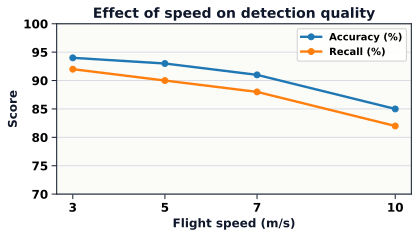
\includegraphics[width=.48\linewidth]{figs/flight_speed.pdf}\label{fig:flight_speed}}
  \\
  \subfloat[Time of day]{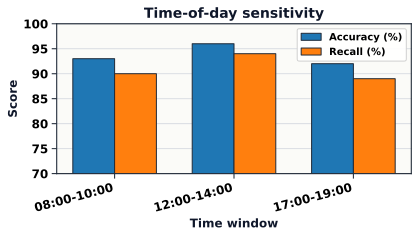
\includegraphics[width=.48\linewidth]{figs/time_of_day.pdf}\label{fig:time_of_day}}
  \hfill
  \subfloat[Weather]{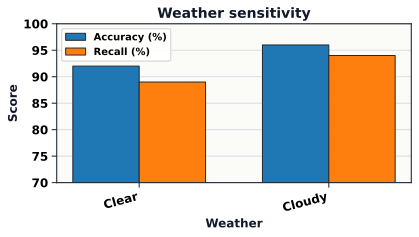
\includegraphics[width=.48\linewidth]{figs/weather.pdf}\label{fig:weather}}
  \caption{Sensitivity of detection performance to operational and environmental parameters. These effects motivate CPS design choices: flight planning and environmental awareness must be part of the system, not afterthoughts.}
  \label{fig:sensitivity}
\end{figure}

\subsection{Quantitative Comparison with Representative State of the Art}
\label{subsec:results_sota}

We compare our results with representative approaches reported in the literature. Direct comparison is imperfect because datasets, defect definitions, and evaluation protocols differ. Nevertheless, Table~\ref{tab:sota} provides a quantitative anchor and clarifies how the proposed CPS differs in scope.

The literature shows that high mAP can be achieved under favorable conditions, for example with ST-YOLO on IR images~\cite{Dey2024STYOLO}. Our ensemble reaches comparable mAP@0.5 for the crack class (0.96) while adding system-level components required for plant operation: geo-indexing, de-duplication, and SCADA-aware decision logic. Multi-stage approaches such as Di Tommaso \textit{et al.} report substantially lower anomaly detection AP@0.5 on hotspots (66.9\%), which illustrates that anomaly detection can be harder than module detection and that dataset and defect type strongly influence metrics~\cite{DiTommaso2022YOLOv3}. Dotenco \textit{et al.} reported strong defect classification performance using classical vision and statistical tests, which remains relevant as a baseline and demonstrates that robust pre-processing is crucial in aerial IR imagery~\cite{Dotenco2016ECCV}.

\begin{table}[!ht]
\centering
\caption{Representative quantitative comparison with published approaches (as reported by the respective authors).}
\label{tab:sota}
\scriptsize
\setlength{\tabcolsep}{3pt}
\begin{tabular}{p{2.7cm}p{1.5cm}p{2.0cm}p{1.8cm}p{1.8cm}}
\toprule
\textbf{Work} & \textbf{Modality} & \textbf{Model / method} & \textbf{Task} & \textbf{Reported metric} \\
\midrule
Dotenco \textit{et al.}~\cite{Dotenco2016ECCV} & IR & Statistical tests + vision & Defect classification & F1 = 93.88\% \\
Di Tommaso \textit{et al.}~\cite{DiTommaso2022YOLOv3} & IR & Multi-stage YOLOv3 & Hotspot detection & AP@0.5 = 66.9\% \\
Dey \textit{et al.}~\cite{Dey2024STYOLO} & IR & ST-YOLO & PV fault detection & mAP@0.5 = 96.6\% \\
\textbf{This work} & IR + RGB & YOLOv11-seg + ensemble + CPS & Defect segmentation + decision & mAP@0.5 up to 96\% (cracks) \\
\bottomrule
\end{tabular}
\end{table}

\begin{figure}[!ht]
\centering
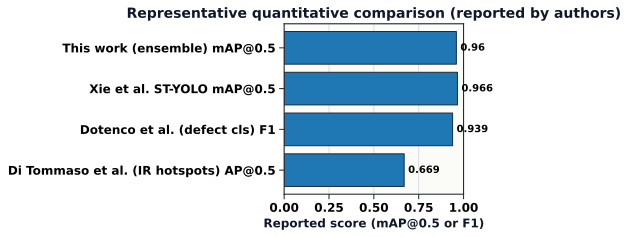
\includegraphics[width=.9\linewidth]{figs/sota_comparison.pdf}
\caption{Representative quantitative comparison (reported metrics). Values are not strictly comparable across datasets; the figure contextualizes the magnitude of results.}
\label{fig:sota_comparison}
\end{figure}

\section{Discussion}
\label{sec:discussion}

The presented results support two intertwined claims. First, a modern segmentation-capable detector can achieve strong defect localization on thermal UAV imagery even with a modest training dataset, provided that post-processing and operational constraints are respected. Second, and more importantly, the operational usefulness of UAV inspection depends on a cyber-physical architecture that connects detection outputs to geo-referenced, de-duplicated events and to plant supervision.

From a computer vision standpoint, the palette-specific results illustrate a subtle but important phenomenon: the thermogram representation is part of the model's input domain. A two-color palette (M2) emphasizes certain gradients and yields stronger crack detection, while a three-color palette (M3) strengthens delamination detection. This is consistent with broader observations in PV thermography that acquisition and rendering choices influence defect contrast and therefore detectability~\cite{Tsanakas2020Review,GallardoSaavedra2020Sensors}. The late-fusion ensemble improves robustness by exploiting this complementarity. The improvement for cracks (0.93 to 0.96 mAP@0.5) is particularly relevant because cracks are often early-stage defects whose thermal signatures can be weak. The runtime reduction (4.235\,s to 2.858\,s) further highlights that engineering the pipeline---not only the network---can yield tangible benefits.

From a systems standpoint, the edge tier is not a luxury. Without RTK-based geo-indexing and de-duplication, raw UAV detections would produce inflated counts and unstable alarms. The architecture therefore treats geo-referencing as a first-class signal, consistent with field studies that emphasize the practical difficulty of mapping anomalies back to modules and strings~\cite{Oliveira2020AerialIR,LeePark2020Sensors}. The edge tier also provides a natural integration point for SCADA signals such as bypass diode status. The Boolean hazard logic (Eqs.~\eqref{eq:fire_logic}--\eqref{eq:fire_logic_ext}) is intentionally interpretable: plant engineers can audit it, adjust it, and embed it in existing rule engines. This contrasts with end-to-end ``black box'' alarm models, which may be difficult to certify for safety monitoring.

The sensitivity analysis offers another argument for the CPS framing. The sharp accuracy drop at 15\,m altitude and at 10\,m/s speed shows that the detector's performance is constrained by physics and optics, not only by model capacity. Similarly, better performance under cloudy conditions suggests that reflections can be a major source of false alarms. These observations motivate the inclusion of reflection-aware planning (Section~\ref{subsec:flightplanning}) and the use of contextual temperature models (Section~\ref{subsec:noct}) as part of the overall system. In other words, the ``best model'' in isolation is insufficient; the system must actively shape its own data through flight planning and quality control.

The proposed approach also has disadvantages and trade-offs. The architecture introduces deployment complexity: an edge server must be maintained on-site, and reliable communication between UAV and edge must be ensured. The approach depends on RTK positioning and on consistent camera calibration; failure in these subsystems can degrade geo-indexing and reduce trust in module-level mapping. The training dataset is relatively small and imbalanced, which may limit generalization to new defect types, new thermal cameras, or different palettes. Although the ensemble improves robustness to palette variation, it also assumes that palette representations are known and consistent; future work should investigate palette-invariant representations or temperature-calibrated models that operate directly on radiometric data rather than rendered palettes.

\paragraph{Limitations, challenges, and open questions.}
Several limitations point to open research directions. First, thermography remains sensitive to environmental conditions; a key challenge is to incorporate irradiance, wind, and ambient temperature into learning models in a principled way, potentially through physics-informed features or uncertainty-aware inference. Second, the current SCADA logic relies on explicit Boolean rules; hybrid approaches that combine learned risk scoring with interpretable rules could improve flexibility while preserving auditability. Third, the geo-indexing step currently uses simplified projection; improving geometric modeling (e.g., through camera calibration and plant 3D models) could reduce association errors in dense plants. Finally, there is a broader question of benchmarking: the PV community would benefit from standardized, publicly available UAV thermography datasets with consistent labels and metadata (flight altitude, irradiance, camera parameters) to enable reproducible comparison across systems.

\section{Conclusion}
\label{sec:conclusion}

This paper presented a method of operating a cyber-physical system for monitoring defects in photovoltaic modules using UAV-based thermography and deep learning, emphasizing that operational adoption depends on architecture and integration rather than on a detector alone. The proposed CPS partitions responsibilities across an on-board UAV tier, an on-site edge tier, and a cloud tier. On-board, a YOLOv11 segmentation model performs real-time defect localization on thermal imagery; on two benchmark thermogram representations (two- and three-color palettes) it achieves macro mAP@0.5 of 0.91 and 0.90, respectively. Late-fusion ensemble across palettes improves the most safety-relevant minority class, increasing crack detection from 0.93 to 0.96 mAP@0.5 and improving delamination detection from 0.93 to 0.95, while also reducing per-frame processing time from 4.235\,s to 2.858\,s. At the system level, RTK-assisted geo-indexing and edge-level de-duplication transform frame-level detections into module-level events suitable for reporting and decision-making. Field validation on rooftop and ground-mounted PV installations yields RMSE of 0.71 between automatic and manual defect counts and shows that operational conditions dominate performance: 10\,m altitude provides a useful trade-off (93\% accuracy, 90\% recall) while 15\,m altitude and 10\,m/s speed substantially degrade recall. The CPS further integrates SCADA-aware fire-risk logic that combines detected defects with bypass diode status and safety sensors in interpretable Boolean rules, enabling transparent alarm generation aligned with plant procedures. Limitations include dataset size and imbalance, dependence on palette representations and RTK accuracy, and sensitivity to reflections and environmental variability. Future work will focus on (i) palette-invariant and radiometric temperature modeling, (ii) uncertainty-aware fusion of thermography with SCADA and weather signals, (iii) improved geometric association of detections to module IDs using calibrated projections and plant digital twins, and (iv) large-scale validation on diverse PV plants to assess generalization and support the creation of standardized UAV thermography benchmarks for reproducible CPS evaluation.

\bibliography{references}

\end{document}
